\documentclass[11pt]{article}

%% PACKAGES
\usepackage{graphicx}
\usepackage[printonlyused]{acronym}
\usepackage{float}
\usepackage[colorlinks=false]{hyperref}
\usepackage{tabularx}
\usepackage{caption}
\usepackage[margin=1.0in]{geometry}
\usepackage{tocloft}
\usepackage{listings}

\lstset{basicstyle=\small\ttfamily,columns=flexible,breaklines=true,xleftmargin=-0.5in,keepspaces=true}

\setcounter{tocdepth}{3}
\setcounter{secnumdepth}{3}

\makeatletter
\g@addto@macro\normalsize{%
  \setlength\abovedisplayskip{0.25pt}
  \setlength\belowdisplayskip{0.25pt}
  \setlength\abovedisplayshortskip{0.25pt}
  \setlength\belowdisplayshortskip{0.25pt}
}
\makeatother

\setlength{\parskip}{\baselineskip}

%% GRAPHICS PATH
\graphicspath{{../../../shared_latex_inputs/images}{../../../shared_latex_inputs/graphs}}

\newcommand{\acposs}[1]{%
	\expandafter\ifx\csname AC@#1\endcsname\AC@used
	\acs{#1}'s%
	\else
	\aclu{#1}'s (\acs{#1}'s)%
	\fi
}

\title{\Huge EMTG Tutorial: Config Files}
\vspace{0.5cm}
\author
{
	Tim Sullivan \thanks{Aerospace Engineer, The Aerospace Corporation}
}
\vspace{0.5cm}

\newcommand{\listofknownissuesname}{\Large List of Known Issues}
\newlistof{knownissues}{mcf}{\listofknownissuesname}

\newcommand{\knownissue}[3]
{
	\refstepcounter{knownissues}
	\par\noindent\textbf{\hyperref[#2_b]{\theknownissues\quad #1}}\label{#2_h}
	\textbf{\hfill\pageref{#2_b}}
	#3
}

\newcommand{\knownissuelabel}[2]
{
	 \phantomsection
  	\hyperref[#2_h]{#1}\def\@currentlabel{\unexpanded{#1}}\label{#2_b}
}

\begin{document}

\begin{titlepage}
\maketitle
\thispagestyle{empty}
\begin{table}[H]
	\centering
	\begin{tabularx}{\textwidth}{|l|l|X|}
		\hline
		\textbf{Revision Date} & \textbf{Author} & \textbf{Description of Change} \\
		\hline
		\date{December 2, 2022} & Tim Sullivan & Initial revision.\\
		\hline
		\date{July 31, 2023} & Joseph Hauerstein & Conversion to \LaTeX.\\ 
		\hline
		\date{August 4, 2023} & Joseph Hauerstein & Addition of Known Issues section.\\ 
		\hline
	\end{tabularx}
\end{table}
\end{titlepage}

\newpage
\tableofcontents
\thispagestyle{empty}
\newpage

\listofknownissues
\thispagestyle{empty}

\knownissue{Apostrophes and quotation marks may not copy to Linux properly}{copy_paste_issue}

\knownissue{PyEMTG does not show that an initial guess has been selected}{no_initial_guess_update_issue}

\knownissue{\acs{PEATSA} plots are not functional}{peatsa_plots_issue}

\knownissue{Output of multiple runs can be written to the same file}{runs_write_to_same_file_issue}

\clearpage
\setcounter{page}{1}



%\section*{List of Acronyms}
\begin{acronym}
%To define the acronym and include it in the list of acronyms: \acro{acronym}{definition}
%To define the acronym and exclude it from the list of acronyms:  \acro{acronym}{definition}
%
%\ac{acronym} Expand and identify the acronym the first time; use only the acronym thereafter
%\acf{acronym} Use the full name of the acronym.
%\acs{acronym} Use the acronym, even before the first corresponding \ac command
%\acl{acronym}  Expand the acronym without using the acronym itself.
%
%

\acro{TCM}{trajectory correction maneuver}
\acro{ACO}{Ant Colony Optimization}
\acro{AD}{Automatic Differentiation}
\acro{ADL}{Architecture Design Laboratory}
\acro{ADM}{asteroid departure maneuver}
\acro{AEI}{atmospheric entry interface}
\acro{AES}{Advanced Exploration Systems}
\acro{AGA}{aerogravity assist}
\acro{ALARA}{As Low As Reasonably Achievable}
\acro{API}{application programming interface}
\acro{BB}{branch and bound}
\acro{BVP}{Boundary Value Problem}
\acro{CATO}{Computer Algorithm for Trajectory Optimization}
\acro{CL}{confidence level}
\acro{CONOPS}{concept of operations}
\acro{COV}{Calculus of Variations}
\acro{D/AV}{Descent/Ascent Vehicle}
\acro{DE}{Differential Evolution}
\acro{RLA}{Right Ascension of Launch Asymptote}
\acro{DLA}{Declination of Launch Asymptote}
\acro{DPTRAJ/ODP}{Double Precision Trajectory and Orbit Determination Program}
\acro{DSH}{Deep Space Habitat}
\acro{DSN}{Deep Space Network}
\acro{DSMPGA}{Dynamic-Size Multiple Population Genetic Algorithm}
\acro{EB}{Evolutionary Branching}
\acro{ECLSS}{environmental control and life support system}
\acro{EGA}{Earth gravity assist}
\acro{ELV}{expendable launch vehicle}
\acro{EMME}{Earth to Mars, Mars to Earth}
\acro{EMMVE}{Earth to Mars, Mars to Venus to Earth}
\acro{EMTG}{Evolutionary Mission Trajectory Generator}
\acro{EVMME}{Earth to Venus to Mars, Mars to Earth}
\acro{EVMMVE}{Earth to Venus to Mars, Mars to Venus to Earth}
\acro{ERRV}{Earth Return Re-entry Vehicle}
\acro{FISO}{Future In-Space Operations}
\acro{FMT}{Fast Mars Transfer}
\acro{GASP}{Gravity Assist Space Pruning}
\acro{GCR}{galactic cosmic radiation}
\acro{GRASP}{Greedy Randomized Adaptive Search Procedure}
\acro{GSFC}{Goddard Space Flight Center}
\acro{GTOC}{Global Trajectory Optimization Competition}
\acro{GTOP}{Global Trajectory Optimization Problem}
\acro{HAT}{Human Architecture Team}
\acro{HGGA}{Hidden Genes Genetic Algorithm}
\acro{IMLEO}{Initial Mass in \acl{LEO}}
\acro{IPOPT}{Interior Point OPTimizer}
\acro{ISS}{International Space Station}
\acro{JHUAPL}{Johns Hopkins University Applied Physics Laboratory}
\acro{JSC}{Johnson Space Center}
\acro{KKT}{Karush-Kuhn-Tucker}
\acro{LEO}{Low Earth Orbit}
\acro{LRTS}{lazy race tree search}
\acro{MAT}{Mars Architecture Team}
\acro{MONTE}{Mission analysis, Operations, and Navigation Toolkit Environment}
\acro{MCTS}{Monte Carlo tree search}
\acro{MGA}{Multiple Gravity Assist}
\acro{MIRAGE}{Multiple Interferometric Ranging Analysis using GPS Ensemble}
\acro{MOGA}{Multi-Objective Genetic Algorithm}
\acro{MOSES}{Multiple Orbit Satellite Encounter Software}
\acro{MPI}{message passing interface}
\acro{MPLM}{Multi-Purpose Logistics Module}
\acro{MSFC}{Marshall Space Flight Center}
\acro{NELLS}{NASA Exhaustive Lambert Lattice Search}
\acro{NMDB}{Navigation and Mission Design Branch}
\acro{NSGA}{Non-Dominated Sorting Genetic Algorithm}
\acro{NSGA-II}{Non-Dominated Sorting Genetic Algorithm II}
\acro{NHATS}{Near-Earth Object Human Space Flight Accessible Targets Study}
\acro{NTP}{Nuclear Thermal Propulsion}
\acro{OD}{orbit determination}
\acro{OOS}{On-Orbit Staging}
\acro{PCC}{Pork Chop Contour}
\acro{PEL}{permissible exposure limits}
\acro{PLATO}{PLAnetary Trajectory Optimization}
\acro{REID}{risk of exposure-induced death}
\acro{RTBP}{Restricted Three Body Problem}
\acro{SA}{Simulated Annealing}
\acro{SLS}{Space Launch System}
\acro{SNOPT}{Sparse Nonlinear OPTimizer}
\acro{SOI}{sphere of influence}
\acro{SPE}{solar particle events}
\acro{SQP}{sequential quadratic programming}
\acro{SRAG}{Space Radiation Analysis Group}
\acro{TEI}{Trans-Earth Injection}
\acro{TIM}{technical interchange meeting}
\acro{TOF}{time of flight}
\acro{TPBVP}{Two Point Boundary Value Problem}
\acro{TMI}{Trans-Mars Injection}
\acro{VARITOP}{Variational calculus Trajectory Optimization Program}
\acro{VGA}{Venus gravity assist}
\acro{VILM}{v-infinity leveraging maneuver}
\acro{MOI}{Mar Orbit Injection}
\acro{PCM}{Pressurized Cargo Module}
\acro{STS}{Space Transportation System}
\acro{EDS}{Earth Departure Stage}
\acro{NEO}{near-Earth asteroid}
\acro{IDC}{Integrated Design Center}
\acro{SEP}{solar-electric propulsion}
\acro{SRP}{solar radiation pressure}
\acro{NEP}{nuclear-electric propulsion}
\acro{REP}{radioisotope-electric propulsion}
\acro{DRM}{Design Reference Missions}

\acro{ASCII}{American Standard Code for Information Interchange}
\acro{AU}{Astronomical Unit}
\acro{BWG}{Beam Waveguides}
\acro{CCB}{Configuration Control Board}
\acro{CMO}{Configuration Management Office}
\acro{CODATA}{Committee on Data for Science and Technology}
\acro{DEEVE}{Dynamically Equivalent Equal Volume Ellipsoid}
\acro{DRA}{Design Reference Asteroid}
\acro{EME2000}{Earth Centered, Earth Mean Equator and Equinox of J2000 (Coordinate Frame)}
\acro{EOP}{Earth Orientation Parameters}
\acro{ET}{Ephemeris Time}
\acro{FDS}{Flight Dynamics System}
\acro{FTP}{File Transfer Protocol}
\acro{GSFC}{Goddard Space Flight Center}
\acro{PI}{Principal Investigator}
\acro{HEF}{High Efficiency}
\acro{IAG}{International Association of Geodesy}
\acro{IAU}{International Astronomical Union}
\acro{IERS}{International Earth Rotation and Reference Systems Service}
\acro{ICRF}{International Celestial Reference Frame}
\acro{ITRF}{International Terrestrial Reference System}
\acro{IOM}{Interoffice Memorandum}
\acro{JD}{Julian Date}
\acro{JPL}{Jet Propulsion Laboratory}
\acro{LM}{Lockheed Martin}
%\acro{LP150Q}{}
%\acros{LP100K}{}
\acro{MAVEN}{Mars Atmosphere and Volatile EvolutioN}
\acro{MJD}{Modified Julian Date}
\acro{MOID}{Minimum Orbit Intersection Distance}
\acro{MPC}{Minor Planet Center}
\acro{NASA}{National Aeronautics and Space Administration}
\acro{NDOSL}{\ac{NASA} Directory of Station Locations}
\acro{NEA}{near-Earth asteroid}
\acro{NEO}{near-Earth object}
\acro{NIO}{Nav IO}
\acro{OSIRIS-REx}{Origins, Spectral Interpretation, Resource Identification, and Security-Regolith Explorer}
\acro{PHA}{Potentially Hazardous Asteroid}
\acro{PHO}{Potentially Hazardous Object}
\acro{SBDB}{Small-Body Database}
\acro{SI}{International System of Units}
\acro{SPICE}{Spacecraft Planet Instrument Camera-matrix Events}
\acro{SPK}{SPICE Kernel}
\acro{SRC}{Sample Return Capsule}
\acro{SSD}{Solar System Dynamics}
\acro{AGI}{Analytical Graphics, Inc.}
\acro{STK}{Systems Tool Kit}
\acro{TAI}{International Atomic Time}
\acro{TBD}{To Be Determined}
\acro{TBR}{To Be Reviewed}
\acro{TCB}{Barycentric Coordinate Time}
\acro{TDB}{Temps Dynamiques Barycentrique, Barycentric Dynamical Time}
\acro{TDT}{Terrestrial Dynamical Time}
\acro{TT}{Terrestrial Time}
\acro{URL}{Uniform Resource Locator}
\acro{UT}{Universal Time}
\acro{UT1}{Universal Time Corrected for Polar Motion}
\acro{UTC}{Coordinated Universal Time}
\acro{USNO}{U. S. Naval Observatory}
\acro{YORP}{Yarkovsky-O'Keefe-Radzievskii-Paddack}

\acro{NLP}{nonlinear program}
\acro{MBH}{monotonic basin hopping}
\acro{MBH-C}{monotonic basin hopping with Cauchy hops}
\acro{FBS}{forward-backward shooting}
\acro{MGALT}{Multiple Gravity Assist with Low-Thrust}
\acro{MGALTS}{Multiple Gravity Assist with Low-Thrust using the Sundman transformation}
\acro{MGA-1DSM}{Multiple Gravity Assist with One Deep Space Maneuver}
\acro{MGAnDSMs}{Multiple Gravity Assist with $n$ Deep-Space Maneuvers using Shooting}
\acro{PSFB}{Parallel Shooting with Finite-Burn}
\acro{PSBI}{Parallel Shooting with Bounded Impulses}
\acro{FBLT}{Finite-Burn Low-Thrust}
\acro{FBLTS}{Finite-Burn Low-Thrust using the Sundman transformation}
\acro{ESA}{European Space Agency}
\acro{ACT}{Advanced Concepts Team}
\acro{IRAD}{independent research and development}
\acro{Isp}[$\text{I}_{sp}$]{specific impulse}
\acro{GA}{genetic algorithm}
\acro{GALLOP}{ Gravity Assisted Low-thrust Local Optimization Program}
\acro{MALTO}{Mission Analysis Low-Thrust Optimization}
\acro{PaGMO}{Parallel Global Multiobjective Optimizer}
\acro{FRA}{feasible region analysis}
\acro{CP}{conditional penalty}
\acro{HOC}{hybrid optimal control}
\acro{HOCP}{hybrid optimal control problem}
\acro{PSO}{particle swarm optimization}
\acro{SEPTOP}{Solar Electric Propulsion Trajectory Optimization Program}
\acro{STOUR}{Satellite Tour Design Program}
\acro{STOUR-LTGA}{Satellite Tour Design Program - Low Thrust, Gravity Assist}
\acro{PaGMO}{Parallel Global Multiobjective Optimizer}
\acro{SDC}{static/dynamic control}
\acro{DDP}{Differential Dynamic Programming}
\acro{HDDP}{Hybrid Differential Dynamic Programming}
\acro{ACT}{Advanced Concepts Team}
\acro{GMAT}{General Mission Analysis Toolkit}
\acro{BOL}{beginning of life}
\acro{EOL}{end of life}
\acro{KSC}{Kennedy Space Center}
\acro{VSI}{variable \ac{Isp}}
\acro{RTG}{radioisotope thermal generator}
\acro{ASRG}{advanced Stirling radiosotope generator}
\acro{ARRM}{Asteroid Robotic Redirect Mission}
\acro{AATS}{Alternative Architecture Trade Study}
\acro{PPU}{power processing unit}
\acro{STM}{state transition matrix}
\acro{MTM}{maneuver transition matrix}
\acro{BCI}{body-centered inertial}
\acro{BCF}{body-centered fixed}
\acro{UTTR}{Utah Test and Training Range}
\acro{EPV}{equatorial projection of $\mathbf{v}_\infty$}
\acro{KBO}{Kuiper belt object}
\acro{DSM}{deep-space maneuver}
\acro{BPT}{body-probe-thrust}
\acro{4PL}{four parameter logistic}
\acro{BCF}{body-centered fixed}

\acro{SPT}{Sun-probe-thrust}
\acro{PIRATE}{PVDrive Interface and Robust Astrodynamic Target Engine}
\acro{PEATSA}{Python EMTG Automated Trade Study Application}
\acro{NEXT}{NASA's Evolutionary Xenon Thruster}
\acro{TAG}{Touch and Go}
\acro{KBO}{Kuiper Belt object}

\acro{CDR}{critical design review}
\acro{PDR}{preliminary design review}
\acro{CCAFS}{Cape Canaveral Air Force Station}

\acro{MRD}{Mission Requirements Document}
\acro{EDL}{entry, descent, and landing}

\acro{Earth-GRAM}{Earth Global Reference Atmospheric Model}
\acro{POST II}{Program to Optimize Simulated Trajectories II}
\acro{MONSTER}{Monte-Carlo Operational Navigation Simulation for Trajectory Evaluation and Research}

\acro{ZSOI}{zero sphere of influence}
\end{acronym}

% --------------------------------------------------------------------------------------------------------------------------
% --------------------------------------------------------------------------------------------------------------------------


%%%%%%%%%%%%%%%%%%%%%
\section{Introduction}
\label{sec:introduction}
%%%%%%%%%%%%%%%%%%%%%

This tutorial provides a brief introduction to the \ac{PEATSA} used for creating and executing \ac{EMTG} trade studies. Example \ac{PEATSA} configuration and output files for this tutorial are provided in the \texttt{EVM\_PEATSA.zip} file included with these tutorials and should be referred to for any questions on setup. For additional details, refer to the PyEMTG User Guide included in \texttt{<EMTG\_root\_dir>/PyEMTG/docs/User\_Guide/PyEMTG\_user\_guide.pdf}. Where \texttt{<EMTG\_root\_dir>} is the directory where you installed \ac{EMTG}.

\noindent \ac{PEATSA} is a set of Python scripts used to create and execute \ac{EMTG} trade studies. \ac{PEATSA} operates by taking an \ac{EMTG} options file, known as the ``base case'', and varying parameters as defined by the user to create and execute variations of the base case. In this tutorial, you will create a \ac{PEATSA} trade study which uses the Earth-Venus-Mars (EVM) trajectory first created in the Boundary Types tutorial and varies the launch date and launch vehicle delta-v upper bound to find the combination of these parameters that yields a trajectory that minimizes the required spacecraft delta-v.

\noindent Unlike previous tutorials which used PyEMTG in a Windows environment, this tutorial will be conducted in Linux entirely through the terminal and text editor. As a consequence, your Linux environment needs to be set up to execute \ac{EMTG}. See the documentation in \texttt{<EMTG\_root\_dir>/docs/0\_ Users/build\_system/linux\_build\_system} for more information.

\noindent\knownissuelabel{NOTE: Be careful if copy/pasting apostrophes and quotation marks from this document to a text editor in a Linux environment. The transcription might not work the way you expect. Inspect each copy/pasted character to ensure it is correct, and change it if necessary.}{copy_paste_issue}

%%%%%%%%%%%%%%%%%%%%%
\section{Setup}
\label{sec:setup}
%%%%%%%%%%%%%%%%%%%%%

Begin with the Journey Boundaries tutorial directory (\texttt{Journey\_Boundaries}). Using your Windows environment, open the \texttt{EVM.emtgopt} \ac{EMTG} options file in PyEMTG. From previous tutorials, you should already have a converged solution for this setup. You can verify that the converged solution produces a feasible trajectory by setting ``Inner-loop Solver Mode'' to ``Evaluate trialX'' in the ``Solver Options'' tab. Then, set the converged solution as the initial guess using the ``Trial decision vector or initial guess'' option and run your options file. You should get a feasible solution. This tutorial will refer to this \ac{EMTG} options file \texttt{EVM.emtgopt} as the \ac{PEATSA} base case.

\noindent\knownissuelabel{NOTE: When selecting the initial guess using the ``Trial decision vector or initial guess'' button, the \acs{GUI} will not update to indicate the selected initial guess has been set, but the new TrialX will have been set in the options file.}{no_initial_guess_update_issue}

\noindent Now, copy the Boundary Types tutorial directory into your Linux environment, including an example solution directory, which should be located in the \texttt{results} folder. In this tutorial, the directory will be named \texttt{EVM} rather than \texttt{Journey\_Boundaries}. From this point on, the \texttt{EVM} directory will be referred to as \texttt{<EVM\_dir>}.

\noindent You also need to copy the \texttt{EVM\_universe} directory to the Linux environment, if it is not contained in \texttt{Journey\_Boundaries}, because you need the \ac{EMTG} universe files and ephemeris data to execute \ac{EMTG}. The directory setup is shown in Figure \ref{fig:evm_directory_setup}.

\noindent The next step is to create a Python script used by \ac{PEATSA} to run the trade study and a trade parameters CSV file which informs \ac{PEATSA} which parameters will be varied and the values to use.

\begin{figure}[H]
	\centering
	\fbox{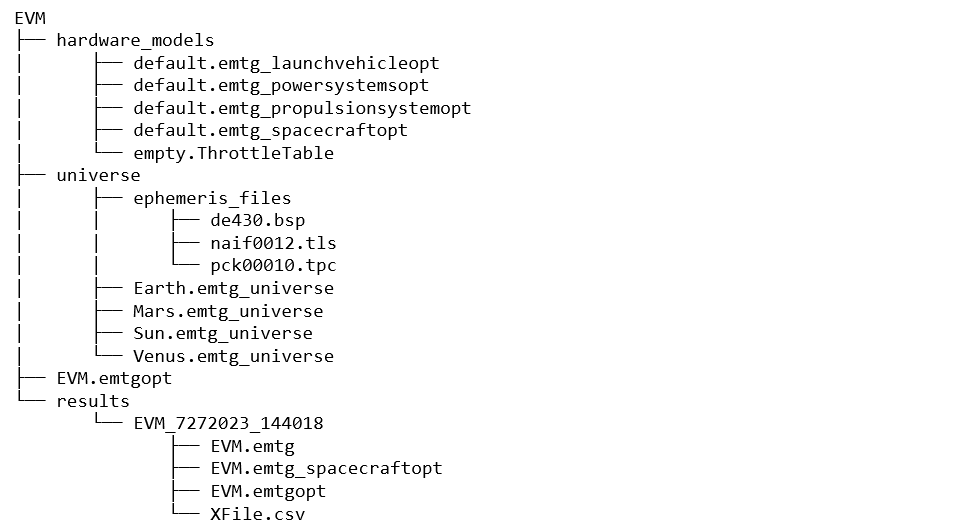
\includegraphics[width=0.9\linewidth]{PEATSA_EVM_directory.png}}
	\caption{\label{fig:evm_directory_setup}\ac{PEATSA} EVM Directory Setup.}
\end{figure}

%%%%%%%%%%%%%%%%%%%%%
\subsection{PEATSA Script Generation}
\label{sec:peatsa_script_generation}
%%%%%%%%%%%%%%%%%%%%%

\ac{EMTG} comes with a Python script to generate the initial \ac{PEATSA} Python file called \texttt{PEATSA\_script \_generator.py}, located in the \texttt{<EMTG\_root\_dir>/PyEMTG/PEATSA} directory. Run the script generator from your \texttt{Journey\_Boundaries} directory with the command:

\texttt{python <EMTG\_root\_dir>/PyEMTG/PEATSA/PEATSA\_script\_generator.py}

\noindent The script generator will begin asking a series of questions in the console and then generate the initial \ac{PEATSA} Python script. Enter the answers listed below to the \ac{PEATSA} script generator. The full question and answer sequence is shown in Figure \ref{fig:script_generation}.

\begin{itemize}
	\item\textbf{How should PEATSA start?} ``Fresh'' -- creating new \ac{PEATSA} cases
	\item\textbf{What type of PEATSA run is this?} ``2'' -- indicates a trade study
	\item\textbf{What is the objective type?} ``0'' -- a new \ac{EMTG} solution is superior to an old solution if the \ac{PEATSA} objective value is better than the old value
	\item\textbf{Should the default plots be generated?} ``0'' -- do not generate default plots

\knownissuelabel{NOTE: Default \ac{PEATSA} plots are not functional at this time. The current workflow is to import \ac{PEATSA} data into software like Excel or Python to perform data analysis and create plots.}{peatsa_plots_issue}
	
	\item\textbf{Filename:} ``\textless EVM\_dir\textgreater /PEATSA\_script.py'' -- include the full path to the mission directory in which the EVM base case was placed
\end{itemize}

\begin{figure}
	\centering
	\fbox{\includegraphics[width=\linewidth]{PEATSA_script_generation.png}}
	\caption{\label{fig:script_generation}\ac{PEATSA} Script Generation.}
\end{figure}

\noindent After answering the script generator questions, you should have a \texttt{PEATSA\_script.py} file in your mission directory. Some additional configuration is required to finish the \ac{PEATSA} run setup. 

\noindent First, a note on PyEMTG objects. Many of the options specified in the \texttt{PEATSA\_script.py} file reference PyEMTG class attributes. Detailed documentation of these options is not yet available. However, users can reference the ``MissionObjects.py'', ``JourneyOptions.py'', ``MissionEvent.py'', and ``Mission.py'' files in \texttt{<EMTG\_root\_dir>/PyEMTG} when configuring different options. In particular, look at the class variables declared in the constructors of these classes to see what data is accessible and the syntax for accessing it. The table below lists a general guide to some of these objects. MissionOptions class attributes are values that define the options for an \ac{EMTG} run; a MissionOptions object is created from a .emtgopt file. On the other hand, Mission class attributes refer to the results of an \ac{EMTG} run; a Mission object is created from a .emtg file. In a \ac{PEATSA} Python script, the MissionOptions and Mission objects for \ac{EMTG} cases are accessed using the shorthand ``MO'' and ``M'', respectively (see Table \ref{tab:pyemtg_objs}). While these options correspond to actual Python objects in PyEMTG, they should be entered in the \texttt{PEATSA\_script.py} file as strings (in quotes), not Python code.


\begin{table}[H]
	\begin{small}
		\begin{tabularx}{\linewidth} { >{\arraybackslash}l >{\arraybackslash} X}
			\hline
			Object & Options/Results Covered \\
			\hline 
			M.& Mission objects (Mission.py) -- Results of an \ac{EMTG} run\newline \\ 
			MO. & Mission options (MissionOptions.py) -- Options used to define an \ac{EMTG} run\newline \\ 
			MO.Journeys[i]. & Journey Options (JourneyOptions.py) -- Options found in the Journey Options panel in PyEMTG\newline \\
			M.Journeys[i]. & Journey results (Journey.py) -- Results from a specific Journey of an \ac{EMTG} run\newline \\
			M.Journey[i].missionevents[j]. & Events within a Journey (missionEvent.py) -- event results from an \ac{EMTG} solution. A mission event corresponds to a row in a .emtg file\newline \\
 			\hline
		\end{tabularx}
	\end{small}
	\caption{\label{tab:pyemtg_objs}PyEMTG Objects.}
\end{table}

\noindent Brackets are used to index array/list elements such as the list of Journeys (every array/list is 0-indexed because Python is 0-indexed).

\noindent\ac{PEATSA} uses ``1'' or ``0'' to indicate True/ON and False/OFF respectively.

\noindent Open \texttt{PEATSA\_script.py} in a text-editor. Make the following changes to the default values set by the script generator:

%%%%%%%%%%%%%%%%%%%%%
\subsubsection{Path Options}
\label{sec:path_options}
%%%%%%%%%%%%%%%%%%%%%

\begin{itemize}
	\item\textbf{run\_name:} ``PEATSA\_run''
	\begin{itemize}
		\item Each time \ac{PEATSA} is run, it will save the results in a directory with this name, appending a number if necessary to avoid overwriting previous results.
	\end{itemize}
	\item\textbf{working\_directory:} the directory containing the \texttt{EVM.emtgopt} file
	\begin{itemize}
		\item This is the directory in which the run\_name folder will be created.
	\end{itemize}
	\item\textbf{nCores:} Set the second element of the tuple to the number of parallel processes you want \ac{PEATSA} to use when executing \ac{EMTG} runs.
	\item\textbf{emtg\_root\_directory:} Full path to the location of the of the EMTG executable.
	\item\textbf{logfile:} Full path and name of file to which \ac{PEATSA} informational output will be written.
\end{itemize}

%%%%%%%%%%%%%%%%%%%%%
\subsubsection{Start Options}
\label{sec:start_options}
%%%%%%%%%%%%%%%%%%%%%

\begin{itemize}
	\item\textbf{max\_iterations:} 2
	\begin{itemize}
		\item This will be set to a low number for this tutorial. After each iteration, the objective formula is evaluated for each case and compared to the best objective achieved in any previous iterations. This information is logged and information about the current iteration is used to seed (provide initial guesses) for the next iteration.
	\end{itemize}
	\item\textbf{if\_run\_cases:} 1
	\begin{itemize}
		\item This tells \ac{PEATSA} to execute \ac{EMTG} cases.
	\end{itemize}
\end{itemize}

%%%%%%%%%%%%%%%%%%%%%
\subsubsection{Initial Case Creation Options}
\label{sec:initial_case_creation_options}
%%%%%%%%%%%%%%%%%%%%%

\begin{itemize}
	\item\textbf{trade\_study\_options\_files:} (``\textless EVM\_dir\textgreater/peatsa\_options.csv'', 1). 
	\begin{itemize}
		\item The list is populated with 2-element tuples. The first element of each tuple is a string containing the full path to a trade parameter CSV, and the second element is an integer specifying the type of the trade parameter CSV. (See Section 3.1.4. of the PyEMTG User Guide). One tuple is inserted into the list with the options file path (this will be created later) and a 1 to trade all values of each variable against all values of all other variables.
	\end{itemize}
\end{itemize}

%%%%%%%%%%%%%%%%%%%%%
\subsubsection{EMTG Control Options}
\label{sec:emtg_control_options}
%%%%%%%%%%%%%%%%%%%%%

\begin{itemize}
	\item\textbf{killtime:} 100 
	\begin{itemize}
		\item This sets a maximum time, in seconds, that an \ac{EMTG} instance is allowed to run before \ac{PEATSA} kills the process. The comments in the \ac{PEATSA} Python file give best practices for setting this value.
	\end{itemize}
	\item\textbf{MBH\_max\_run\_time:} 60
	\begin{itemize}
		\item This defines how long in seconds each case is allowed to run in \ac{EMTG}. Note that this value will be superseded if \texttt{MBH\_max\_run\_time} is set in the override\_options, described later and in Section 3.1.3 of the PyEMTG User Guide.
	\end{itemize}
\end{itemize}

\noindent The killtime variable is required because \ac{SNOPT} can encounter an unrecoverable failure that causes an \ac{EMTG} run to never end, even if \texttt{MBH\_max\_run\_time} is exceeded.

%%%%%%%%%%%%%%%%%%%%%
\subsubsection{Optimization Options}
\label{sec:optimization_options}
%%%%%%%%%%%%%%%%%%%%%

\begin{itemize}
	\item\textbf{objective\_formula:} ``M.total\_deterministic\_deltav''
	\begin{itemize}
		\item This sets the \ac{PEATSA} objective value; that is, how \ac{PEATSA} decides if one \ac{EMTG} run is better than another. The formula must be a function of data that is obtainable from a PyEMTG Mission object and MissionOptions object for a given \ac{EMTG} run. Note that this objective value does not have to be the same as the objective function for a single \ac{EMTG} run.
	\end{itemize}
	\item\textbf{max\_or\_min:} ``min'' 
	\begin{itemize}
		\item You want to minimize total delta-v.
	\end{itemize}
\end{itemize}

%%%%%%%%%%%%%%%%%%%%%
\subsubsection{Sorting Options}
\label{sec:sorting_options}
%%%%%%%%%%%%%%%%%%%%%

\begin{itemize}
	\item\textbf{fingerprint:} [``MO.launch\_window\_open\_date'', ``MO.Journeys[0].initial\_impulse\_bounds[1]'']
	\begin{itemize}
		\item The list of strings in the fingerprint defines a unique \ac{EMTG} case. A good starting point is to make the fingerprint a list of the trade parameter column headers.
		\item These will set in the options CSV file later in the tutorial. The \ac{PEATSA} run you create will vary the start of the launch window and the upper bounds on the impulse imparted by the launch vehicle to see what impact these have on the spacecraft delta-v.
	\end{itemize}
	\item\textbf{seed\_from\_cases\_that\_havent\_met\_target:} 1
	\begin{itemize}
		\item This variable defaults to 0 but typically should be 1. When 0/OFF \ac{EMTG} will not seed new cases from previous runs unless the objective value has been reached. It’s common to set the objective value to 0 or a very high number for minimization/maximization problems, respectively, such as minimizing delta-v or maximizing dry mass. \ac{EMTG} solutions will rarely achieve these values, meaning previous runs will never be used as seeds for new runs. This is usually not the desired behavior since \ac{PEATSA} should select previous runs as initial guesses for future runs.
	\end{itemize}
	\item\textbf{only\_one\_seed\_in\_all\_seed\_directions:} 1
	\begin{itemize}
		\item\knownissuelabel{NOTE: If you have multiple seed criteria, multiple \ac{PEATSA} runs may be seeded by the same previous run, with each run given the same name. This means that multiple runs will be written to the same file. This causes problems parsing the solution. If this bug has been fixed, the value can be set to 0 or 1 at the user’s discretion. If the seed\_criteria list (see below) has only a single entry, then setting to 0 or 1 is OK.}{runs_write_to_same_file_issue}
	\end{itemize}
	\item\textbf{seed\_criteria:} [(``MO.launch\_window\_open\_date'', -30.1, 30.1, 2),\newline (``MO.Journeys[0].initial\_impulse\_bounds[1]'', -1.1, 1.1, 2)]
	\begin{itemize}
		\item For case A to be a potential seed for case B, case A’s fingerprint must be identical to case B’s fingerprint except for the value of the seed criterion element under evaluation. This list specifies the range for a seed criterion in which a previous run is allowed to serve as a seed for a future run.
		\item This list is made up of 4-element tuples. The first element is a string that is the criterion to be compared between an \ac{EMTG} case and a potential seed case. This should be a trade parameter as defined in the trade parameters CSV file. (See Section 3.1.4 of the PyEMTG User Guide.) The second element is a real number that is the maximum negative seed range. In other words, when evaluating a potential seed case, how much less than the current case can the seed criterion be for the seed case to still be considered a potential seed? The third element is a real number that is the maximum positive seed range. In other words, when evaluating a potential seed case, how much greater than the current case can the seed criterion be for the seed case and still be considered a potential seed? The fourth element is an integer and is the seed selection criterion.
		\item The values above indicate that a previous run launch window open date can be used as a seed for 30 days in either direction, and that the initial impulse upper bound can be used as a seed for 1.1 km/s above or below the seed run’s value. The upper and lower values in the seed criteria were selected to slightly overlap adjacent values set in the options CSV file. The [0] and [1] indicate that parameter is indexing an array or tuple. (In this case, Journeys[0] is indexing into the list of JourneyOptions objects and initial\_impulse\_bounds[1] is grabbing the upper bound on the initial impulse.
	\end{itemize}
	\item\textbf{override\_options:} [(``1'', ``MO.HardwarePath = `\textless EVM\_dir\textgreater /hardware\_models/' ''), (``1'', ``MO.universe\_folder = `\textless EVM\_dir\textgreater /universe/' ''), (``1'', ``MO.run\_inner\_loop = 1''), (``1'', ``MO.seed\_MBH = 1'')]
	\begin{itemize}
		\item This list is used to override \ac{EMTG} options from the base case. For example, the base case might be generated in Windows using PyEMTG, and this section can be used for a \ac{PEATSA} run on a Linux server on multiple cores by overriding the paths to the universe and hardware directories. The list should be comprised of two-element tuples where the first element is a logical condition that, when it evaluates to true, indicates the override should be applied. To always apply the override, place a ``1'' as the first element. The second element is an assignment statement indicating what option to override and the value to assign it.
		\item For this tutorial, add override options for the universe and hardware directories because you are running on a different system than the system on which you created the base case, and the base case file paths are not present on the linux system. If your most recent run of your base case set ``Inner-loop Solver Mode'' to something other than ``Monotonic Basin Hopping'', then you will also want to override that (1 corresponds to monotonic basin hopping for \texttt{run\_inner\_loop}). You also want to make sure that seeding \acs{MBH} is turned on. See Section 3.1.3 of the PyEMTG User Guide for more options.
	\end{itemize}
\end{itemize}

%%%%%%%%%%%%%%%%%%%%%
\subsubsection{Post-Processing Options}
\label{sec:post_processing_options}
%%%%%%%%%%%%%%%%%%%%%

\begin{itemize}
	\item\textbf{extra\_csv\_column\_definitions:} [(``C3(\(\mathrm{km^2/s^2}\))'', ``M.Journeys[0].missionevents[0].C3''),\newline (``Launch Date'', ``M.Journeys[0].missionevents[0].GregorianDate''),\newline (``Launch Date'', ``M.Journeys[0].missionevents[0].JulianDate'')]
	\begin{itemize}
		\item After each \ac{PEATSA} iteration, \ac{PEATSA} produces a CSV file that summarizes the results of each \ac{EMTG} run in a single file. This section allows the user to add columns to the IterationX.csv output files produced by \ac{PEATSA} and is used to show more information about the solutions \ac{EMTG} finds and/or the options used for an \ac{EMTG} run. A column is added by adding a two-element tuple to the extra CSV column definitions. The first element is a string defining the column header. The second element is a string that may be evaluated for a given \ac{EMTG} run. Data must be obtainable from a PyEMTG Mission object or MissionOptions object for a given \ac{EMTG} run. These objects are accessed via ``M.'' and ``MO.'', respectively.
	\end{itemize}
\end{itemize}

%%%%%%%%%%%%%%%%%%%%%
\subsection{PEATSA Trade Parameters File}
\label{sec:peatsa_trade_parameters_file}
%%%%%%%%%%%%%%%%%%%%%

This tutorial has referred several times to a CSV file that defines trade study parameters. Now you will make that file. This file can be made in Excel and saved as a CSV or any text editor with careful attention to formatting. (Using Excel is usually easier because it handles formatting automatically.) There are three types of trade parameter files that can be used in \ac{PEATSA}. You will be using ``Type 1'', which trades all values of each variable against all values of all other variables. In other words, an \ac{EMTG} case is created for every permutation of the values listed in rows 4 and below of the CSV (see the PyEMTG User Guide Section 3.1.4 for more information).

\noindent The first row of the CSV should contain the full path to the base case directory. The second row should contain the file name to the base case \ac{EMTG} options file located in the directory in row 1. In other words, when the file name in row 2 is appended to the directory path in row 1, you get the complete path to the base \ac{EMTG} options file. (The first row entry does not need to end with a file separation character.) The third row should contain the names of the trade parameters used for the \ac{PEATSA} run. Set these to \texttt{MO.launch\_window\_open\_date} and \texttt{MO.Journeys[0].initial\_impulse\_bounds[1]}. The [1] indicates the upper bound value and the [0] indicates this applies to the first Journey. Thus, the trade parameters are the earliest date the spacecraft is allowed to launch, and the maximum impulse allowed to be provided by the launch vehicle.

\noindent Rows 4 and below contain the values to be tested for each of the parameters labeled in row 3. For \texttt{MO.launch\_window\_open\_date}, set the value in row 4 to 61041, which is the modified Julian date for 1 January 2026. In the rows below, enter additional Julian dates spaced 30 days apart. (Note that this value of 30 days is set in conjunction with the value for the upper bound of ``Wait time bounds'' for Journey 0 of the base case, which is set to be slightly greater than 30 days.) Thus, you will be attempting to launch in 30-day ``bins''. For \texttt{initial\_impulse\_bounds[1]}, begin with 5 km/s and increase by 1 km/s in each row. Add as many rows as you like, remembering that the total runs will scale with the product of the number of values in each column. The spacing for both corresponds to the values set in seed criteria. 

\noindent NOTE: The gap between launch window open dates in this tutorial is 30 days so that a year of launch dates can be examined with a small number of \ac{EMTG} cases. In practice, however, the gap is usually set to a smaller value, such as 5 days, in order to make ``adjacent'' cases have similar enough solutions that using a feasible solution for one case as an initial guess for an adjacent case is likely to result in a new feasible case after optimization is performed. In general, proper selection of the distance between adjacent values of trade parameters is important in order for \ac{PEATSA} to fully take advantage of its seeding capabilities.

\noindent If editing this file using a text editor, ensure there are commas between values in each row with no spaces and no empty lines below the trade parameter values. If either of these are present, \ac{PEATSA} will throw an error at runtime. If using Excel, saving the file as a CSV should result in a correctly formatted options file.

\noindent Save your CSV. Remember that the path to and name of the CSV need to be consistent with the value given to \texttt{trade\_study\_options\_files} in the \ac{PEATSA} Python file. An example file is shown in Figure \ref{fig:trade_param_file_ex}.

\begin{figure}
	\centering
	\fbox{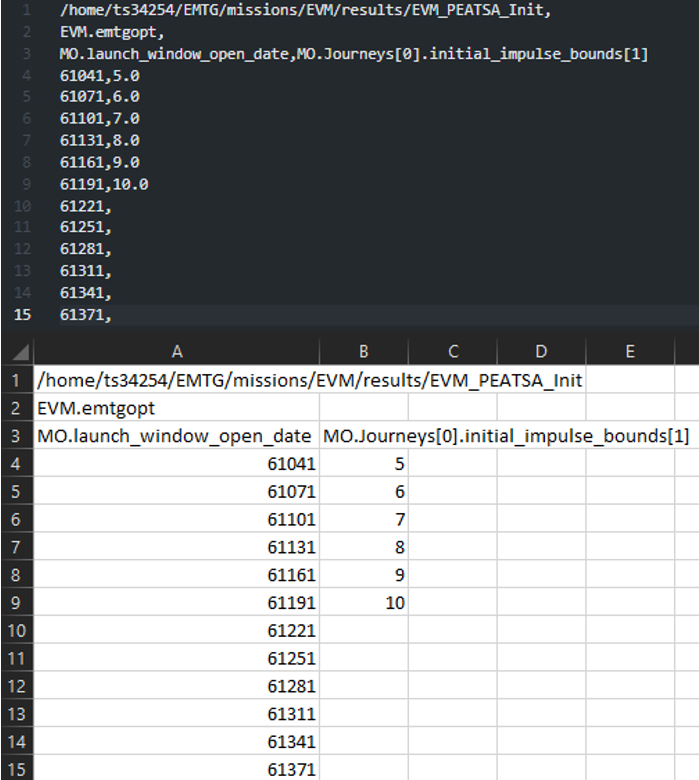
\includegraphics[width=0.9\linewidth]{PEATSA_trade_parameter_file_examples.png}}
	\caption{\label{fig:trade_param_file_ex}Trade Parameter CSV File Examples.}
\end{figure}


%%%%%%%%%%%%%%%%%%%%%
\section{Run PEATSA}
\label{sec:run_peatsa}
%%%%%%%%%%%%%%%%%%%%%

Once the files required to set up a \ac{PEATSA} run have been created, the Linux command to execute a \ac{PEATSA} run is (all on one line):

\texttt{nohup python <EMTG\_root\_dir>/PyEMTG/PEATA/PEATSA.py <EVM\_dir>/PEATSA\_script.py >\newline\indent /path/to/terminal.out 2>\&1 \&}

\noindent This command will:

\begin{itemize}
	\item Use Python to execute \texttt{PEATSA.py} with \texttt{PEATSA\_script.py} as a command-line argument.
	\item Ignore the hang-up signal so that the process does not stop if the user logs out or is disconnected (\texttt{nohup}).
	\item Redirect standard output and standard error to a file named \texttt{terminal.out} (\texttt{> /path/to/term inal.out 2>\&1}). \ac{PEATSA} writes output to this file, so the user can monitor the progress of a \ac{PEATSA} run by examining the contents of this file or the file set for the \texttt{logfile} variable in the \ac{PEATSA} Python setup script. The user can also see if a \ac{PEATSA} run has died unexpectedly by examining this file. Keep in mind that once \ac{PEATSA} finds the \texttt{logfile}, it will only output to that file.
	\item Run in the background (\texttt{\&}).
\end{itemize}
\noindent As soon as the \ac{PEATSA} run is kicked off, the folder set for \texttt{run\_name} should be created. You can follow the progress of your \ac{PEATSA} run at its most basic level using the Linux \texttt{top} command. You should see python and/or \ac{EMTG} process(es) being executed if everything is going well. More detailed logging information can be seen by looking at the contents of the \texttt{logfile} using the command:

\texttt{tail -f /path/to/logfile}


%%%%%%%%%%%%%%%%%%%%%
\section{Post-Process}
\label{sec:post_process}
%%%%%%%%%%%%%%%%%%%%%

\ac{PEATSA} runs produce a lot of files. Figure \ref{fig:example_peatsa_run_dir} shows a reduced example of the contents of a \ac{PEATSA} output directory with \texttt{run\_name = "PEATSA\_run"} after two \ac{PEATSA} iterations (iteration 0 and iteration 1). Each case that \ac{PEATSA} creates for \ac{PEATSA} iteration X results in a new \ac{EMTG} options file placed in the \texttt{cases/IterationX} directory. The normal \ac{EMTG} output is placed in the \texttt{results/IterationX} directory. You’ll note that the filenames include which preceding case seeded the current case. A summary of the results for each iteration will be placed in an \texttt{IterationX.csv} file in the docs directory. The \texttt{PEATSAhistory.csv} file, also in the docs directory, provides basic summary information such as the how many \ac{EMTG} runs executed, how many converged, how many failed, and how many improved. This can be useful for determining whether a \ac{PEATSA} run should be stopped, adjusted, and/or restarted. The file is overwritten after each iteration, so it always provides up-to-date information from all the iterations prior the current one. An example is shown in Table \ref{tab:peatsa_history}.

\noindent The \texttt{IterationX.csv} file contains the seed criteria used for each run, \ac{PEATSA} objective, additional columns we set above, and other information. There is one row for each unique fingerprint of the trade study, and its contents represent the best solution that \ac{PEATSA} has found for that fingerprint in any \ac{PEATSA} iteration up to and including iteration X. The \ac{EMTG} results themselves are in \texttt{PEATSA\_run/results/IterationX} and the \ac{EMTG} options file for each case are in \texttt{PEATSA\_run/cases/IterationX}.

\begin{figure}[H]
	\centering
	\fbox{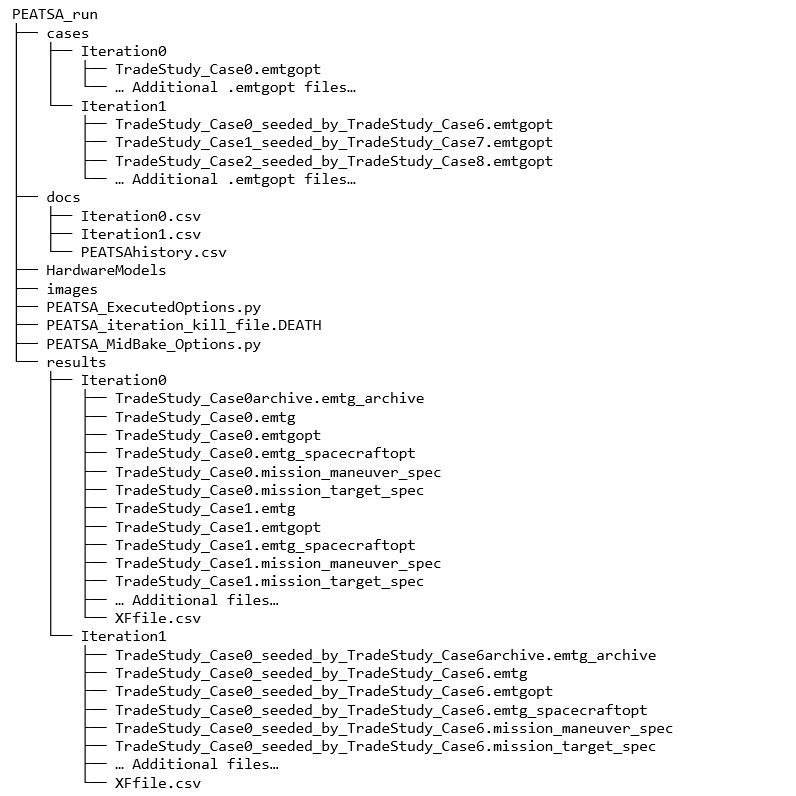
\includegraphics[width=\linewidth]{PEATSA_example_run_directory.png}}
	\caption{\label{fig:example_peatsa_run_dir}Example \ac{PEATSA} Run Directory.}
\end{figure}

\begin{table}[H]
	\begin{small}
		\begin{tabularx}{\linewidth} { >{\arraybackslash}X >{\arraybackslash} l >{\arraybackslash} l}
			\hline
			Iteration & 0 & 1 \\
			Cases Created & 72 & 72 \\ 
			Cases Run & 72 & 72 \\ 
			Ran Unseeded & 72 & 0 \\
			Cases Finished & 72 & 71 \\
			Iteration Cases Converged & 72 & 71 \\
			\ac{PEATSA} Cases Converged & 72 & 72 \\
			First Convergence this Iteration & 72 & 0 \\
			Improvement this Iteration & 72 & 39 \\
			Number of \ac{PEATSA} Cases That Converged on First \acs{NLP} Solve This Iteration & 36 & 71 \\
			Average Number of Solution Attempts for all Cases This Iteration & 546.89 & 533.75 \\
			Average Solution Attempt Number of BEst Feasible Solution Amoung All Feasible Cases This Iteration & 277.21 & 201.75 \\
			Times Using Seed Before Improvement & 72 & 6 \\
 			\hline
		\end{tabularx}
	\end{small}
	\caption{\label{tab:peatsa_history}Example \texttt{PEATSAhistory.csv} Contents.}
\end{table}

\noindent The \texttt{IterationX.csv} files are especially useful for exploring and presenting the trade space. Add as many custom columns as necessary to understand the advantages and disadvantages of different mission configurations using the \texttt{extra\_csv\_column\_definitions} list. For our Earth-Venus-Mars case, Figure \ref{fig:run_results} can be created using the iterations file, looking at the spacecraft delta-v required for different combinations of launch vehicle C3 (characteristic energy, the square of V-infinity which we traded in this \ac{PEATSA} run) and launch date. Be careful -- Rows of the \texttt{IterationX.csv} file whose \texttt{Filename} column starts with FAILURE did not converge and should be filtered out of any analyses. 

\begin{figure}[H]
	\centering
	\fbox{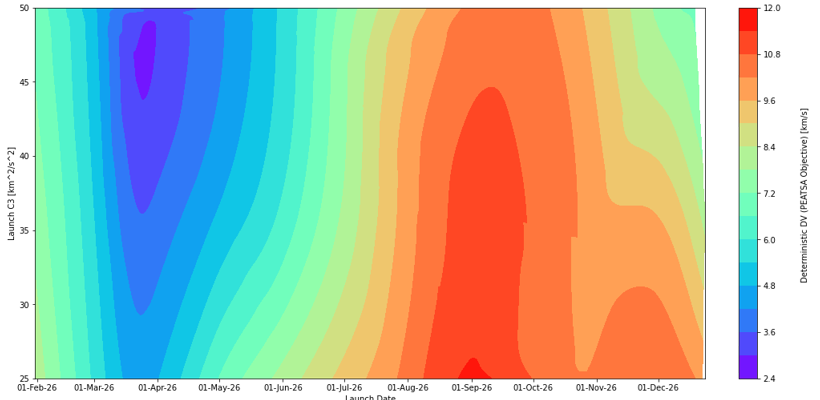
\includegraphics[width=\linewidth]{PEATSA_run_results.png}}
	\caption{\label{fig:run_results}\ac{PEATSA} Run Results.}
\end{figure}


%%%%%%%%%%%%%%%%%%%%%
\subsection{Best Results}
\label{sec:best_results}
%%%%%%%%%%%%%%%%%%%%%

\noindent\ac{PEATSA} includes another script, \texttt{<EMTG\_root\_dir>/PyEMTG/PEATSA/grab\_best\_peatsa\_results. py}, which will fetch the feasible case with the best \ac{PEATSA} objective for each fingerprint and place them in a user-defined folder. The command syntax for this script is:

\texttt{python <EMTG\_root\_dir>/PyEMTG/PEATSA/grab\_best\_peatsa\_results.py /path/to/PEATSA\newline\indent\_run/ /path/to/best\_peatsa}

\noindent Where \texttt{/path/to/PEATSA\_run} is the directory from which to extract results and \texttt{/path/to/best\_pea tsa} is the destination for the best feasible cases. These results can be used to seed a new \ac{PEATSA} case and reduce disk usage by filtering out ``bad'' cases, but note that iteration CSV files are not saved by this command, so be careful deleting old run directories. Note that the script does not create \texttt{/path/to/best\_peatsa}; you must create it ahead of time.

\noindent This concludes the introductory tutorial on \ac{PEATSA}! \ac{PEATSA} contains capabilities beyond what was discussed. Refer to the PyEMTG User Guide, the comments in the \ac{PEATSA} script created by the script generator, and the PyEMTG options files listed in Section \ref{sec:peatsa_script_generation} to learn more about PEATSA’s capabilities.


\end{document}